\subsection{Scale: the gap does not grow when every arm has its own learning rate}\label{sec:scale}
An earlier exploratory screen of ours (Appendix~\ref{app:laneme}) found that the device gap grows with width once the FP
learning rate is re-tuned per width. If true, that would be a serious obstacle, so we tested it directly.

\paragraph{Design.}
\begin{itemize}
\item Widths: CIFAR base channels $c\in\{16,32,64\}$ and LM widths $d\in\{64,128,256\}$, with a fixed training budget.
\item Arms: FP; and TTv2 and \RETwoBestchopped{} on the protonic and Li-ECRAM devices.
\item Learning rates: every arm chooses its own on validation at every width, with the edge rule.
\item Seeds: three test seeds per arm and width.
\item Verdict: GROWS, SHRINKS or FLAT, by the pre-registered rule (Section~\ref{sec:protocol}).
\end{itemize}

\paragraph{Result} (Table~\ref{tab:scale}, Fig.~\ref{fig:scale}).
\begin{itemize}
\item Of \REFourNArms{} device--algorithm arms, \REFourNGrows{} GROW, \REFourNFlat{} are FLAT and \REFourNShrinks{} SHRINK.
      The two that shrink are TTv2 on the LM, for both devices.
\item The earlier observation is therefore \textbf{\REFourConfirmed}.
\item On the LM the tuned device arms are \emph{better} than FP-SGD, and increasingly so at width 256. The protonic device with
      \RETwoBestchopped{} is \REFourLmProtonicOnenTwoZeroTwoTwoCttvTwoWTwoFiveSixGap\% at $d=256$ and
      \REFourLmProtonicOnenTwoZeroTwoTwoCttvTwoWOneTwoEightGap\% at $d=128$.
\end{itemize}

\paragraph{Why the earlier screen saw growth.}
\begin{itemize}
\item The earlier runs, like our specification sweep (Section~\ref{sec:spec}), used the \emph{FP} learning rate for the device.
\item At width 64 (CIFAR) and 256 (LM) that rate is a poor choice for a Tiki-Taka device. The base protonic device with TTv2 at
      the FP rate has a gap of \RSpecrelTtvTwoCifarWSixFourBasegap\,pp and \RSpecrelTtvTwoLmWTwoFiveSixBasegap\%.
\item At its own rate (TTv2: \REFourCifarProtonicOnenTwoZeroTwoTwoTtvTwoWSixFourGap\,pp and
      \REFourLmProtonicOnenTwoZeroTwoTwoTtvTwoWTwoFiveSixGap\%) the gap is gone.
\item The device arms chose rates up to \REFourLrRatioMax$\times$ above FP's. TTv2's two-array structure filters the gradient like a leaky
      accumulator, the analogy to momentum drawn by~\cite{rasch2024}, and tolerates larger steps.
\end{itemize}

\paragraph{Caveats.}
\begin{itemize}
\item Our FP baseline is plain SGD at a fixed budget. At $d=256$ its validation-chosen rate
      ($\REFourLmFplrWTwoFiveSix$) leaves it at \REFourLmFpWTwoFiveSix{} bits per byte, worse than at $d=128$
      (\REFourLmFpWOneTwoEight). Part of the analog arms' advantage at $d=256$ is FP-SGD's under-training at this budget, not an
      analog gain.
\item Three widths spanning a factor of four are a small range. Our conclusion is limited to it: we find no evidence that the
      gap grows with width once learning rates are tuned per arm.
\end{itemize}

% generated by analyze.py (do not edit)
\begin{table*}[t]\centering\footnotesize\caption{Scale (E4): every arm uses its own validation-chosen learning rate (in parentheses) at every width; gap (pp for CIFAR, \% for the LM), mean and 95\% interval over 3 seeds paired with FP at its own learning rate. Verdict by the pre-registered rule (Section~\ref{sec:scale}).}\label{tab:scale}
\fitbox{\begin{tabular}{llccccc}\toprule Task & Width & FP metric (lr) & Li-ECRAM c-TTv2 & Li-ECRAM TTv2 & Protonic c-TTv2 & Protonic TTv2\\\midrule
CIFAR & 16 & 55.70 (0.0003) & 0.64 [-1.53, 2.82] (0.003) & 1.86 [-0.64, 4.35] (0.001) & -2.13 [-7.14, 2.88] (0.003) & 0.41 [-1.44, 2.26] (0.001)\\
CIFAR & 32 & 60.15 (0.001) & -0.40 [-3.13, 2.33] (0.001) & 2.12 [-1.66, 5.90] (0.001) & -1.88 [-6.35, 2.59] (0.003) & -0.21 [-5.27, 4.84] (0.003)\\
CIFAR & 64 & 60.87 (0.0003) & -1.34 [-5.57, 2.89] (0.001) & 1.11 [0.17, 2.05] (0.001) & -1.30 [-3.56, 0.96] (0.003) & 0.33 [-2.43, 3.09] (0.001)\\
\multicolumn{3}{r}{verdict:} & FLAT & FLAT & FLAT & FLAT\\\midrule
LM & 64 & 3.193 (0.0001) & -0.55 [-8.58, 7.48] (0.0001) & -0.31 [-6.26, 5.63] (0.0003) & -7.21 [-11.77, -2.65] (0.0003) & -3.45 [-6.44, -0.46] (0.0003)\\
LM & 128 & 2.881 (0.0001) & -0.09 [-7.23, 7.04] (0.0001) & -0.60 [-8.73, 7.53] (0.0003) & -6.38 [-12.53, -0.23] (0.0003) & -3.88 [-10.90, 3.14] (0.0003)\\
LM & 256 & 3.100 (3e-05) & -13.73 [-14.66, -12.79] (0.0001) & -9.01 [-10.21, -7.82] (0.0001) & -12.97 [-13.57, -12.36] (0.0001) & -8.48 [-9.67, -7.29] (0.0001)\\
\multicolumn{3}{r}{verdict:} & FLAT & SHRINKS & FLAT & SHRINKS\\
\bottomrule\end{tabular}}\end{table*}

\begin{figure}[t]\centering
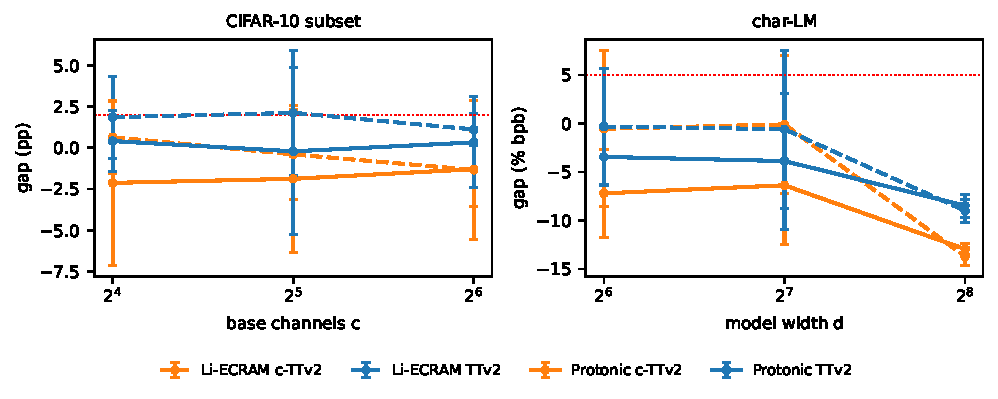
\includegraphics[width=\linewidth]{figs/fig_scale}
\caption{Gap against width with every arm at its own validation-chosen learning rate (mean and 95\% interval, 3 seeds); solid:
protonic, dashed: Li-ECRAM; dotted: the gap line.}\label{fig:scale}
\end{figure}
